\chapter{Introduction}

% Slightly copy from Itay Erez's thesis? Or simply cite it?
% Explain in more detail about our candidates and from there talk about IVR


\section{What are Chiral Molecules?}

\section{Our Experimental Scheme}

% Explain about our the general scheme, or cite something?
% Explain about our ion trap in details, especially details relevant to the velocity / kinetic energy resolution required and hence the maximal temperatures required.
% Show the level diagram for Yb+ and from there justify the need for a 935nm LASER 
% Comparison to typical molecular ion trapping setups

\section{All Trapping \& Cooling Parameters}

The experimental scheme described above justifies optimizing the cooling process, and hence invite the main effort and research topic of this thesis - simulations of the trapping and (sympathetic) cooling our molecule. The simulations were performed by LAMMPS\cite{LAMMPS}, which is capable of simulating numerous classical models relevant in many contexts, but in our case, I chose a simple model of charged point particles with only long-range coulomb interactions, and an electrical field resembling the field generated by our ion trap, along with a velocity dependent force imitating the LASER cooling. Justifying the resemblance of the trapping and cooling parameters in real life to the simulation's code is detailed in the subsections below.

\subsection{Trapping}\label{ssec:params-trapping}

% TODO: Decide whether to present the naive_freqs and micromotion parameters. The offset_{x,y,z} parameters should probably be presented.

Simulating real-life electrodes and their interactions with charged particles is very hard, and LAMMPS is incapable of doing that. There are software tools out there that use Finite elements methods that are capable (e.g \cite{FEniCS}) of performing such calculations, but they are limited to electrostatics, and calculating dynamics with them would require immense effort and probably high computing resources. Hence, in this research effort, I took an analytical expression for a time varying quadrupole electric field, that is relatively easily inserted into LAMMPS, that implements the ion trap.\footnote{A potential advantage for using analytical expressions, is the ability to study the effects of higher order terms of the electric potential - terms that further limit the validity of the harmonic approximation, which will be explained in subsequent paragraphs. Studying these effects could be a topic for further research, and it is out of scope for this research.}

In contrast to SIMION\cite{SIMION}, and possibly many more electrodynamics simulating tools, LAMMPS \emph{is} calculating Coulomb interactions, along with interactions to the external electric field, largely thanks to the fact it is given in an analytical expression. It should be noted that besides neglecting boundary effects, LAMMPS is also neglecting magnetic fields induced by simply the movement of the ions.

The basic form of the electric field in axis $i \in {x,y,z}$, inserted in the simulations is of the following form:

$$ E_i = (a_i + q_i \cos(2\pi f_{rf} t)) x_i$$

Where the dimensions of $a_i$ and $q_i$ are naturally $\mathrm{Volt}/\mathrm{distance^2}$. In strong contrast to common derivations of the Mathieu equations from geometric properties of the electrodes that implement the trap, this analysis is purely analytical. It \emph{is} possible to obtain a grid of electric potential values, using a software tool that solves the Laplace\footnote{And not Poisson!} equation, and then try to fit the model above to the electric fields obtained. However, that has proved to be rather difficult, especially for all spatial axes together (in contrast to the slightly easier fitting experience of a 1 dimensional $\phi(x_i)$ slice). Additionally, there is no way to predict accurately the effect of changing voltages of the electrodes upon the grid of voltages.

Hence, it was decided to avoid justifying a relation of the analytical expression to the physical design of the trap, and instead focus on the implementation of finding a set of $(a_i, q_i)$ with $i \in {x,y,z}$ such that certain secular frequencies are obtained from the Mathieu equations. The Mathieu equation of axis $i$ can be formulated like this:
% TODO: Cite at the end of the above sentence an article that solves Mathieu

\begin{equation}
	\gamma_{n+1} + \gamma_{n-1} = \frac{\tilde{a}_i - \left(\beta_i + n\right)^2}{\tilde{q}_i} \gamma_n,\quad \forall i\in\{x,y,z\},\ \forall n\in\mathcal{Z}
\end{equation}

Where $\beta_i \equiv 2 f_{\mathrm{secular}(i)}/f_{rf}$ is the normalized secular frequency, $\tilde{a}_i/a_i = \tilde{q_i}/q_i = \alpha$ is a constant factor, and $\gamma_n$ are vector elements of a non-trivial solution to the infinite system of equations. Additionally the following 2 Laplace equations must be satisfied too:

\begin{equation}
	\sum_{i\in{x,y,z}} a_i = \sum_{i\in{x,y,z}} q_i = 0
\end{equation}

Altogether, we have 5 equations, and 6 unknowns. The last equation required to determine a single possible solution, can be:

\begin{equation}
	q_z = 0
\end{equation}

% TODO: Add a citation for an example of a q_z = 0 in literature, and better explain why this is justified for us too.
This slightly arbitrary equation is weakly justified for most ion traps observed in literature. In our trap design too, it makes sense because...

% TODO: Consider writing a more thorough derivation in the Computational Challenges chapter

\subsection{Cooling}

The theory of LASER cooling is well established for 2-level systems. The semi-classical model implemented in the simulations presented in this work is explained well in literature\cite{TannoudjiCooling,SteckCooling} and can be expressed as follows:

\begin{equation}
	\mathbf{F}(\mathbf{v}) = \frac{h \pi \gamma \hat{k}}{\lambda} \cdot \frac{\omega^2/2}{1/4 + \omega^2/2 + (d - \hat{k}\cdot\mathbf{v}/\lambda/\gamma)^2}
\end{equation}

Where:

\begin{itemize}
	\item $h$ is Planck's constant.
	\item $\hat{k}$ is the LASER's spatial direction.
	\item $\lambda$ is the cooling transition.
	\item $\gamma$, is the cooling transition's lifetime in Hz dimensions. The more commonly used $\mathrm{rad}/\mathrm{s}$ scaled lifetime is usually denoted as $\Gamma = 2\pi \gamma$.
	\item $d$ is the LASER's detuning normalized to $\Gamma$. Sometimes the not normalized detuning in the dimensions of $\mathrm{rad}/\mathrm{sec}$ is denoted as $\delta$ and with it we can denote $d \equiv \delta/\Gamma$.
	\item $\mathbf{v}$ is the velocity of the cooled Atom.
	\item $\omega$ is the LASER's Rabi frequency normalized to $\Gamma/2\pi$. Very similarly to $d$ and $\delta$ the following can be stated: $\omega \equiv \Omega/\Gamma$.
\end{itemize}

In principal, there is a Taylor expansion for the above expression for low $\mathbf{v}/\lambda/\gamma$. Let's observe this expansion for a slightly simplified, 1 spatial dimensional form of the force - with $\mathbf{v} = (v,0,0)$ and $\hat{k} = (1,0,0)$:

\begin{equation}
	\frac{h \pi \gamma}{\lambda} \cdot \frac{\omega^2/2}{1/4 + \omega^2/2 + d^2} \left(
		1 + \frac{2d}{1/4 + \omega^2/2 + d^2} \cdot v/\lambda/\gamma
	\right)
	\label{eq:laser-cool-taylor-force}
\end{equation}

To understand the effect of the 0th order force component, let's observe a simplistic system of a 1 dimensional harmonic oscillator with a damping force of the form above:

\begin{equation}
	\ddot{x} = - \omega_{sec}^2 x + F_0/m - 2 \xi \omega_{sec} \dot{x}
\end{equation}

Where $\omega_{sec}$ is the secular frequency well defined by our trap as explained in subsection \ref{ssec:params-trapping} and $\xi$ is derived from the 1st order force component in expression \ref{eq:laser-cool-taylor-force}. The well known solution is of the form: 

\begin{equation}
	x(t) = \frac{F_0}{m \omega_{sec}^2} + A e^{-\xi \omega_{sec} t} \sin(\sqrt{1-\xi^2}\ \omega_{sec} t + \phi)
\end{equation}

Where $A$ and $\phi$ are determined by initial conditions. The steady state's offset from the origin $F_0/m\omega_{sec}^2$ in the case of a LASER cooling force equals:

\begin{equation}
x_o = \frac{h \pi \gamma}{\lambda}\cdot\frac{\omega^2/2}{1/4+\omega^2/2 + d^2} \cdot\frac{1}{m \omega_{sec}^2}
\end{equation}

If we'll take:

\begin{itemize}
	\item Secular frequency $\omega_{sec}$ in the order of magnitude of $\sim 2\pi\cdot 1.5\mathrm{kHz}$.
	\item LASER intensity of $\omega \equiv \Omega/\Gamma = 1$. % TODO: Consider writing a footnote or something mentioning what is the relation to actual mW/cm^2 \footnote{The relation}
	\item A common LASER detuning of $d \equiv \delta/\Gamma = 1/2$. % TODO: Cite or footnote why is this considered common.
	\item \ce{Yb^+} and the cooling transition at $c/\lambda = 811.2891 \mathrm{THz}$ with the linewidth $\Gamma/2\pi \equiv \gamma = 19.6 \mathrm{MHz}$. % TODO: \cite{YbCoolingThesis} Anthony Ransford's thesis
\end{itemize}

% TODO: Is this really true?
We'd get $x_o \approx 2.1 \mathrm{mm}$, where the trap's harmonic region is of about $25 \mathrm{mm}$ from the origin. This offset might not be very significant for only LASER cooling a single ion like \ce{Yb^+}, but sympathetic cooling will suffer from this offset, as the target molecule won't experience an identical offsetting force, and would not collide frequently enough with the cooling and lose energy this way. Naturally increasing the secular frequencies of the trap greatly reduces this offset, but our trap's design doesn't allow much higher secular frequencies.

% TODO: Consider citing and discuss a bit about what kind of forces other people use in simulations - discuss with Yuval about the fact the real expression for any \hat{k} and \mathbf{v} includes many cross-terms and looks very messy.

% TODO: Ask Yuval whether more references for using counter-propagating beams would be useful here:
As suggested in a more classical LASER cooling model presented by Dan Steck\cite{SteckClassicalCooling}, we can use 2 counter propagating LASER beams, that will apply 2 forces which sum up to $\mathbf{F}(\mathbf{v}) - \mathbf{F}(-\mathbf{v})$, forming an odd function, with no 0th order Taylor coefficient. Creating 2 such counter-propagating beams in experiment is simply done with a mirror. However, the vacuum chamber's windows induce an small attenuation on the intensity, as illustrated in figure \ref{fig:windows-attenuation}.

\begin{figure}[h!]
	\begin{center}
		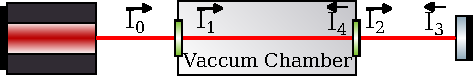
\includegraphics[width=0.95\textwidth]{graphics/windows-attenuation.pdf}
	\end{center}
	\caption{The effect of the Vaccum Chamber's windows' attenuation upon the LASER cooling intensities.}\label{fig:windows-attenuation}
\end{figure}

Since $\omega \equiv \Omega/\Gamma$ and $I \propto \Omega^2$, if we'd define\footnote{The experimentalist's most intuitive measurement is to measure $I_2/I_0$, but it should be equal $I_4/I_1$ assuming all windows are made of identical glass, and the intensity lost in the mirror is 0.} $\alpha \equiv I_4/I_1$, the actual force we are imposed to apply upon our ions is:

\begin{equation}
	\mathbf{F}(\mathbf{v}, \omega) - \mathbf{F}(-\mathbf{v}, \sqrt{\alpha}\omega)
\end{equation}

Causing a slight imperfect oddness (with respect to $\mathbf{v}$) of the force, depending on the windows attenuation parameter $\alpha$.

\subsubsection{Summery}

This is a good place to pause and list all the simulation parameters we collected from the theory above:

\begin{itemize}
	\item The LASER cooled ion. Choosing an ion and a cooling transition is effectively choosing $\lambda$, $\gamma$ and the mass $m$.\footnote{Cooling transitions and line-widths were taken from \cite{CoolingBeParameters,CoolingCaParameters1,CoolingCaParameters2,RansfordThesis,RadiumData}}. Current experimental efforts as well as all simulations presented focus on \ce{Yb^+}, but in principal this parameter is not hard-coded, and 
	\item The normalized LASER's intensity $\omega \equiv \Omega/\Gamma$.
	\item The normalized LASER's detuning $d \equiv \delta/\Gamma$.
	\item The spatial direction(s) of the LASER(s). This can be parameterized by a list of $(\theta, \phi)$ pairs - a pair per LASER, defining each LASER's $\hat{k}$ using a spherical coordinates transformation.
	% TODO: Consider whether adding this
	%\item Whether to use the approximated Taylor expression with only the 1st order term. This is not really a physical simulation parameter, but it was studied because I couldn't find simulations simulations in literature not using the approximation.
	\item The Vacuum chamber's windows' attenuation. Our experiment's attenuation is $\alpha = 0.7$, and most simulations use this value.\footnote{Besides figure ... which displays it's effect.}
	% TODO: \ref{fig:windows-attenuation-effect} in the results
\end{itemize}

Lastly, the relation of the Rabi frequency $\Omega$ to the actual LASER intensity\cite{CJFootOmega2I}, is worth mentioning\footnote{The software is capable of displaying $\omega$ dependence in the scale of the intensity $I$, but this behavior wasn't activated in the results presented.}:
% TODO: Make sure the above footnote is correct

\begin{equation}
	I = \frac{2\pi h c \Gamma}{3 \lambda^3} \cdot \left(\frac{\Omega}{\Gamma}\right)^2
\end{equation}

\subsection{Time Periods}

To fully define a simulation, one has to define a few more parameters. Two of which are related to the timeline and are referred to as cooling and stabilizing time. The cooling time period has trivial meaning and increasing it can be interesting but naturally the price is higher computing resources demands. The stabilization time is the time since $t=0$ up to the point where the LASER cooling force enters. For researching cooling parameters, and for most initial temperatures, there is no need for more then $5-7\mathrm{ms}$ of stabilizing time, just to let the thermodynamic instabilities of the initial conditions minimize. Figure \ref{TODO1} can serve as a good example in which the width of $T(t)$ before the LASER cooling starts decreases enough after $5 \mathrm{ms}$.

\label{TODO1}

Another usage for varying the stabilization time, is for measuring the eigenfrequencies of the trap, without cooling ($0$ cooling time), and all cooling parameters irrelevant.

\subsection{Time Dividing Finesse}

Another fairly technical parameter is the finesse of the time division. As further justified in subsection \ref{ssec:T_rf_type}, we want to always divide the simulation to an integer number of RF cycles. Since the RF frequency is also the highest frequency of the system, the natural thing to do is to divide each RF cycle to an integer number of steps, and this slightly arbitrary parameter is called the RF divisor. There is no theory that predicts an optimal RF divisor, and still this is a rather important technical detail:

One can perform many simulations with a certain RF divisor, and only in a specific simulation, in a specific advanced time, notice a certain ion has experienced a non-physically strong Coulomb force, causing it to fly way very far away, making the temperatures measurements noisy throughout the rest of the simulation, and hence essentially incorrect. With way too low RF divisors the temperatures measurements will be noisy and incorrect from the start. After a few months of optimizing this parameter, a value for the RF divisor was stabilized around $\sim 1500$. To further tighten the demand of the RF division's independence from potential numerical errors, a prime number was chosen.\cite{primesieve} More examples demonstrating effects of low RF divisors, and hence proving convergence for RF divisors $\sim 1500$, are available in section \ref{sec:comp/coulomb}.
% TODO: The above ref may need to be updated.

\subsection{Initial Conditions}

Lastly, the initial conditions were obtained using a random number generator with a specific seed. Each seed integer represents a reproducible set of initial conditions, given the algorithm distributing positions and velocities stays the same. To decouple the (small) effects of initial conditions upon the results, the same simulations but with different seeds were ran, and in most results displayed this dimension was averaged over.

% Put all the onenote's technical challenges related content here

\section{Output Result Types}

Naturally, the main result that interests us is the temperature. Which is essentially a common measure for the average kinetic energy, and in our case, since we use a VMI, it is a measure of the velocities' distribution's width. A physically related property of our ion clouds is the size, that can be measured per axis simply via a \texttt{std}. As for the temperatures, there are a few more ways to measure them, laid out below. 

\subsection{Temperature's Random Variables}

Under the approximated treatment of the Ion trap's potential as a perfect harmonic potential, and with the long range Coulomb potential neglected, one can treat the positions analogously, and hence almost identically to the velocities. This is done by multiplying each particle's position $x_i$ in the $i$'th axis, by $2\pi f_i x_i$, where $f_i$ is the secular frequency of the Ion trap in the $i$'th axis.\footnote{Although not implied by an existence of an additional index besides $i$, there is a different, non-trivial set of $f_i$ secular frequencies per particle species, as described in section \ref{ssec:params-trapping}.}
% TODO: Make sure the above ref is specific as possible

% TODO: Use labels per these temperatures related subsections, and \ref to them in the technical part of the thesis.
\subsection{Temperature's Probabilistic Methods}

Given $N$ particles, which were 'measured' during the computer simulation in a certain time, 2 arrays of shapes \texttt{(N,3)} are obtained for velocities and positions. The positions' array can be scaled by the proper secular frequencies as described above, and the question of how to compute a temperature given such an array has multiple legitimate answers. To layout all available answers we'll denote the random variable $u_i \in \{v_i, 2\pi f_i x_i\}$ for axis $i$. The $i$'th slice of length \texttt{N} from the above \texttt{(N,3)} shaped array is a distribution of the $u_i$ random variable.

One simple answer which is most intuitive in the context of VMI based measurements is to simply compute $m \mathrm{Var}(u_i)/K_\text{B}$, as derived from the Maxwell-Boltzmann distribution expression:

\begin{equation}
	f(\mathbf{u}) \mathrm{d}^{3}\mathbf{u} = \left[\frac{m}{2\pi k_{\text{B}}T}\right]^{3/2}\,\exp \left(-{\frac {m \mathbf{u}^2}{2K_\text{B} T}}\right) \mathrm{d}^{3}\mathbf{u}
\end{equation}

Another approach, is to integrate over a solid angle of $\mathbf{u}$ in the probabilistic model above, and write a speeds-like distribution function:

\begin{equation}
	f(|\mathbf{u}|) = \left[{\frac{m}{2\pi K_\text{B} T}}\right]^{3/2} 4\pi |\mathbf{u}|^{2}\exp\left(-{\frac{m |\mathbf{u}|^{2}}{2k_{\text{B}}T}}\right)
\end{equation}

Which has a variance equal to $K_\text{B} T/m \cdot (3 - 8/\pi)$, and a squared mean equal to $K_\text{B} T/m \cdot 8/\pi$, thus providing 2 more methods to calculate a temperature given a \texttt{(N,3)} shaped array of either positions or velocities.

\subsection{Temperature Under the Secular Approximation}\label{ssec:T_rf_type}

In addition to the velocities and/or positions choice of random variable(s), and in addition to the above probabilistic model approaches, one has to decide how to imitate the secular approximation computationally. The physical justification for doing it, is the fact that in a crystal phase (which we aim achieving), the movement of the ions is strongly coupled to the RF field which we have direct control over. Essentially the model states that the collective movement due to the RF field is predictable and so well defined, that it is not a random variable.

Experimentally speaking, we are capable of measuring positions and velocities always at the beginning/end of each RF cycle, and hence always use an integer number of RF cycles. This is the simplest and probably the only way of implementing a secular approximation experimentally, and it should work best for ions that have formed a crystal. In the following, we'll describe what other techniques are available to a computer simulation that might help achieve time dependent, secularly approximated temperature measurements.\footnote{There's also a technical motivation to imitate some kind of secular approximation when measuring temperatures, and that is reducing the amount of disk writes required when simulating $\sim 3,000$ RF cycles divided to $\sim 1500$ time steps. Reducing the amount of disk writes not only reduces disk usage of simulation result files, but also speeds up the total time required for simulating.}

% TODO: Cite stuff from zothero regarding RF averaging..
Besides sampling the velocities and positions in the beginning of each RF cycle, many simulations based research found in literature average over an RF period each particle's per-axis velocity, and then construct a temperature. You might hope that the same can be done for $2\pi f_i x_i$, but apparently, even for ion clouds initiated in a thermal gas phase equilibrium in temperatures as low as $5\mathrm{K}$, each particle reaches many spatial areas of the trap, and it's RF averaged position produce (incorrect) temperatures in the $\mathrm{\mu K}$ regime! This proves that this approach is not accurate also for the velocities, at least for gas like phases, as it suggests that ions go through a big part of the phase-space. Never the less, I decided to do save the RF averaged velocities (but not the positions) to the disk during simulations, and the software displaying the simulation results provides the option to use this data.

Another interesting RF cycles related option, is to sample the velocities and positions in the middle of each RF cycle - where the kinetic energy induces by the RF field should be at it's peak. The difference from the energies in the beginning of the RF cycles may help extract the RF motion energy. This data was also saved for both positions and velocities, for consistency.

\subsection{Temperatures Options Summary}\label{ssec:T-options-summery}

The above temperatures related options are modeled in software as 3 dimensions with the names and symbolic optional values as defined in table \ref{tbl:T_methods}

\begin{table}
\begin{tabular}{l||l|l|l|l|l}
Dimension   & \multicolumn{5}{c}{Optional values}\\
\hline\hline
% TODO: Maybe T_coord is not a good name?
 \texttt{T\_coord}   & $\vec{v}$                                    & \multicolumn{2}{l}{$\overrightarrow{\omega x}$} \\
\hline
\texttt{T\_rf\_type} & $\left\langle\circlearrowright\right\rangle$ & $\mathrm{min}\left(\circlearrowright\right)$ & \multicolumn{2}{l}{$\mathrm{max}\left(\circlearrowright\right)$} \\
\hline
\texttt{T\_method}  & $\mathrm{Ave}\left(|u|\right)^2(\pi/8)$      & $\mathrm{Var}\left(|u|\right)/(3 - 8/\pi)$   & $\mathrm{Var}\left(u_x\right)$               & $\mathrm{Var}\left(u_y\right)$ & $\mathrm{Var}\left(u_z\right)$ \\
\hline
\end{tabular}
\caption{Ways to measure temperatures, obtained from a generalized maxwell-Boltzmann model}
\label{tbl:T_methods}
\end{table}

Where $\circlearrowright$ marks an RF cycle, and $\left\langle\circlearrowright\right\rangle$ marks an average over RF cycle. The functions $\mathrm{Ave}$ and $\mathrm{Var}$ operate upon a 1 dimensional array of length $N$ - the number of particles sampled.

Lastly, we can select specific, multiple temperature values and average over the different methods, coordinates and RF methods. A common example is to take the positions and velocities sampled in the beginning of each RF cycle ($\mathrm{min}\left(\circlearrowright\right)$), and calculate the temperature according to all the \texttt{T\_method}s. Whatever specific \texttt{T\_coord}s / \texttt{T\_rf\_type}s / \texttt{T\_method}s were chosen, the code analyzing and displaying the simulation results averages over these dimensions while keeping the time dependence of course.\footnote{Technically, the temperatures obtained from the RF averaged ($\left\langle\circlearrowright\right\rangle$) positions ($\overrightarrow{\omega x}$) are considered \texttt{NaN} and hence ignored.}

\subsection{Further Summarizing Analyzes}

Up until now we discussed time dependent properties of our ion clouds - the per spatial axis size and the various temperatures. We can also summarize these results to obtain various measures of how fast did we cool our ions, and how much smaller did the cloud get due to the LASER cooling etc. This is termed both in the code and here as summarized results.

The simplest summarized result type is the temperature/size after the cooling process, which is defined (slightly arbitrarily) as the average temperature/size of the ion cloud in the last 1/4 of the time before cooling or before the end. The first \textit{part} is referred to as \textit{stabilizing part} and the later \textit{cooling part}. The standard deviation of the temperature/size in each such \textit{part} defines the uncertainty for each such summarized measurement. The size measurement, both in the time dependent form and in the summarized form depends on the spatial axis (x,y,z), and the temperatures, in either the summarized or time dependent form, depend on the 3 dimensions described in subsection \ref{ssec:T-options-summery}.

Another summarized measurement is the cooling frequency, defined (for simplicity, only for temperatures) as follows: Given a $T(t)$ defined using any of the parameters of subsection \ref{ssec:T-options-summery}, we take $Log(T(t)/\mathrm{kelvin})$, and apply a continuous piecewise linear fit\cite{pwlf}, with 2 segments. This gives 2 cooling frequencies in the units of $\mathrm{kHz}$ that depend on a dimension referred to as \texttt{regime}. This design choice stems from the observation that in many simulations most of the ion cloud is cooled quickly and efficiently whereas afterwards the rest of the cooling happens in a mixed thermodynamic phase of an ion crystal (massive and highly charged) with a gas of ions surrounding it. The initial, faster and more efficient part of the cooling process corresponds to the 1st segment of exponential temperature decay, and the rest of the cooling is significantly slower, and hence invite defining a 2nd segment of cooling.

Lastly, only for verifying the frequencies expected from the Mathieu equations of the ion trap, as explained in subsection \ref{ssec:params-trapping}, we define the following analysis referred to as the \textit{cloud's frequencies}: Given the time dependent positions of all ions, we average over the ions to get the cloud's center position (still time and spatial axis dependent). With it, we can take the Fourier transform and get the dominant frequency via \texttt{scipy.signal.find\_peaks}\cite{scipy}, or simply via \texttt{numpy.argmax}\cite{numpy}. If the collective movement is very harmonic (due to e.g collective offset in which the ion cloud was intentionally placed at $t=0$), a fit for a $\cos(2\pi f x_i + \phi)$ can be attempted, and the fit's frequency is the dominant frequency of movement. The time range of the simulation dictates the uncertainty in the dominant frequency obtained via a Fourier transform, and the dominant frequency of the fit produces uncertainties via the covariance matrix returned by \texttt{scipy.optimize.curve\_fit}.
